\documentclass[10pt,letterpaper]{article}
\usepackage[left=.71in,right=.71in,top=.57in,bottom=.60in]{geometry}
\usepackage[T1]{fontenc}
\usepackage{mathptmx,graphicx,xcolor,booktabs,tabularx,array,hyperref}
\hypersetup{hidelinks,pdftitle={GEAR-Nav: two uses for the extra page}}
\pagestyle{empty}
\setlength{\parindent}{0pt}
\setlength{\parskip}{5pt}
\definecolor{rust}{HTML}{944823}
\definecolor{slate}{HTML}{445668}
\newcommand{\option}[2]{{\sffamily\small\bfseries\color{rust}#1}\par
  \vspace{2pt}{\fontsize{22}{25}\selectfont\bfseries #2\par}}
\newcommand{\subhead}[1]{\par\vspace{3pt}{\large\bfseries #1}\par}
\newcommand{\source}[2]{{\small\color{slate}\href{#1}{#2}}}

\begin{document}
{\sffamily\small\bfseries\color{rust}OPTION A \enspace/\enspace HELD-OUT VIDEO}
\par\smallskip
\noindent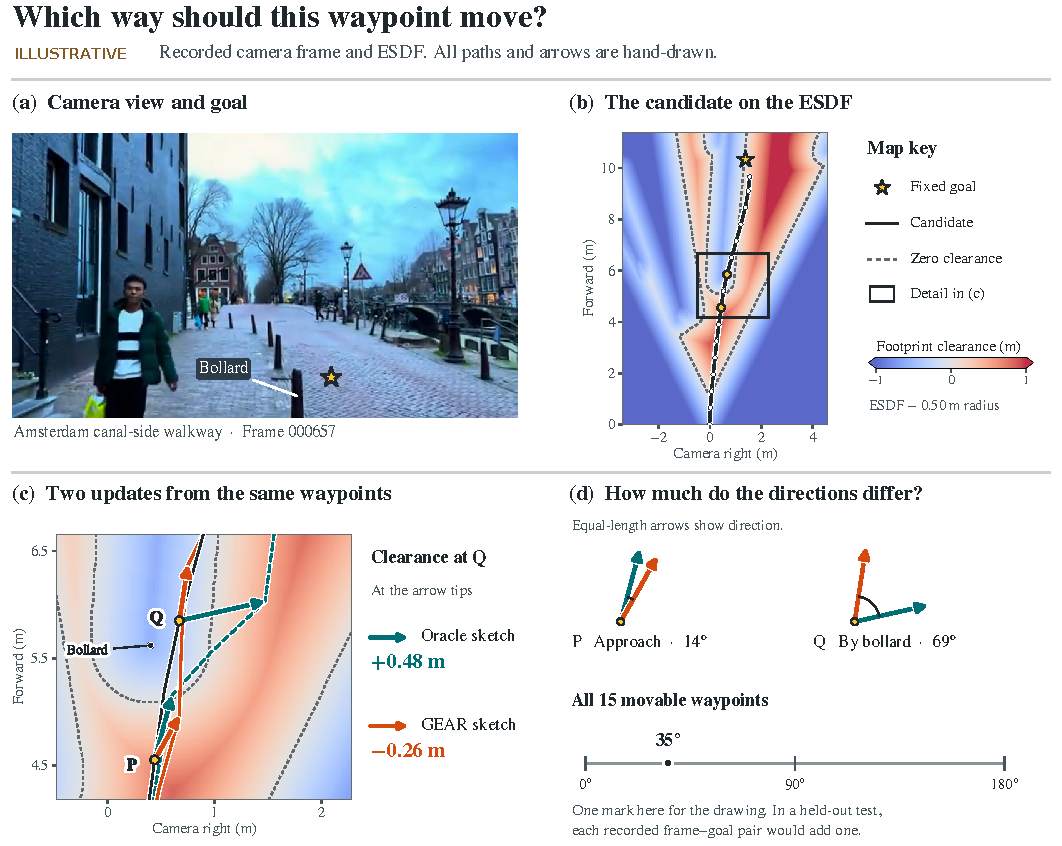
\includegraphics[width=\linewidth]{illustrative_update/illustrative_update.pdf}

\subhead{What an endpoint comparison would miss}
The two hand-drawn proposals finish at the same point. On the open approach (P), their updates point in nearly the same direction. Beside the bollard (Q), the teal arrow carries the waypoint to the clear side of the footprint boundary. The orange arrow moves mostly forward and stays inside it. The clearance readings come from the recorded map at the two drawn arrowheads. The ESDF treats unobserved space as occupied.

\subhead{What this would test in the paper}
Figure~1 shows a path evolving through repeated updates. Here the camera, goal and candidate would all be held fixed. For example, take the candidate after seven model updates on each held-out frame--goal pair. Ask the oracle and the action head for their next update at that exact path. Panel~(d) would then show one angle per pair, computed over the displacements of all 15 movable waypoints. Cases with a zero-length update would be counted separately. The comparison belongs beside the held-out evaluation in Sec.~V-D.

\vfill
{\small\color{slate}Recorded source: Amsterdam\_3, frame 000657, sampled goal 1.
\source{https://www.youtube.com/watch?v=ABuu-odtMOk&t=3880s}{Source video at 1:04:40.}
Paths, arrows and angle examples are illustrative.}
\newpage
\option{OPTION B \enspace/\enspace PHYSICAL ROBOT}{What happens as a pedestrian passes?}
Follow one Vision~60 trial from the approaching pedestrian to the scooter goal. The four timestamps come from one continuous external-camera recording of hardware Scenario~3.

\begin{center}
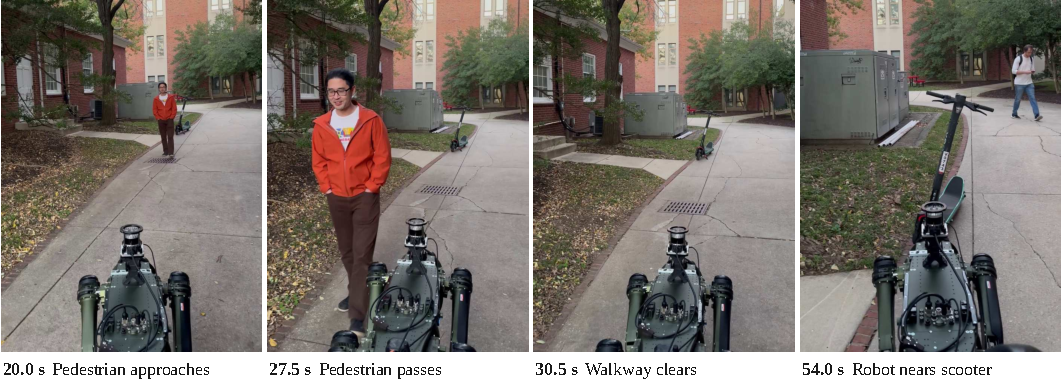
\includegraphics[width=\linewidth]{../navigation_results/pedestrian_pass.pdf}
\end{center}

\subhead{Read the sequence against all three routes}
The film strip shows one successful case. The trial counts show where the robot also struggled. Hardware success requires arrival within 0.5\,m without contact or safety intervention. Each row therefore partitions its 20 runs into three outcomes.

\vspace{3pt}
\begin{tabularx}{\linewidth}{@{}Xrrr@{}}
\toprule
Hardware target & Success & Contact or intervention & Other unsuccessful trials\\
\midrule
Person (Scenario 1) & 16 & 4 & 0\\
Blue chair (Scenario 2) & 16 & 0 & 4\\
Scooter (Scenario 3) & 20 & 0 & 0\\
\bottomrule
\end{tabularx}
\par\vspace{5pt}
The two 16/20 outcomes have different explanations at the level of the recorded metrics. Every unsuccessful trial on the person route involved contact or intervention. All four unsuccessful trials on the blue-chair route ended without a recorded collision.

\subhead{What the reader can see}
The pedestrian passes before the robot nears the scooter. The frames establish the event order. A synchronized plot of the robot's local waypoint predictions would be needed to say how the action head changed the path during the encounter.

\subhead{Where it fits}
Place the sequence next to the physical-robot discussion in Sec.~V-B. iPlanner links successive planning events to onboard observations and local trajectories. ViPlanner uses a similar sequence to explain why two planners behave differently at the same site. \source{https://www.roboticsproceedings.org/rss19/p064.pdf}{iPlanner, Fig.~1.} \source{https://arxiv.org/pdf/2310.00982}{ViPlanner, Fig.~5.}

\vfill
{\small\color{slate}Recording: Scene 3, IMG\_4546.MOV. Counts derived from the existing hardware table.}
\end{document}
